%%%%%%%%%%%%%%%%%%%%%%%%%%%%%%%%%%%%%%%%%%%%
\section{My lines of research}


{
\paper{\textbf{M. Xochicale 2019} PhD thesis, DOI:10.5281/zenodo.3384145}
\begin{frame}{Movement Variability in HRI using nonlinear dynamics}
    \vspace{-00mm}
      \begin{figure}
        \centering
        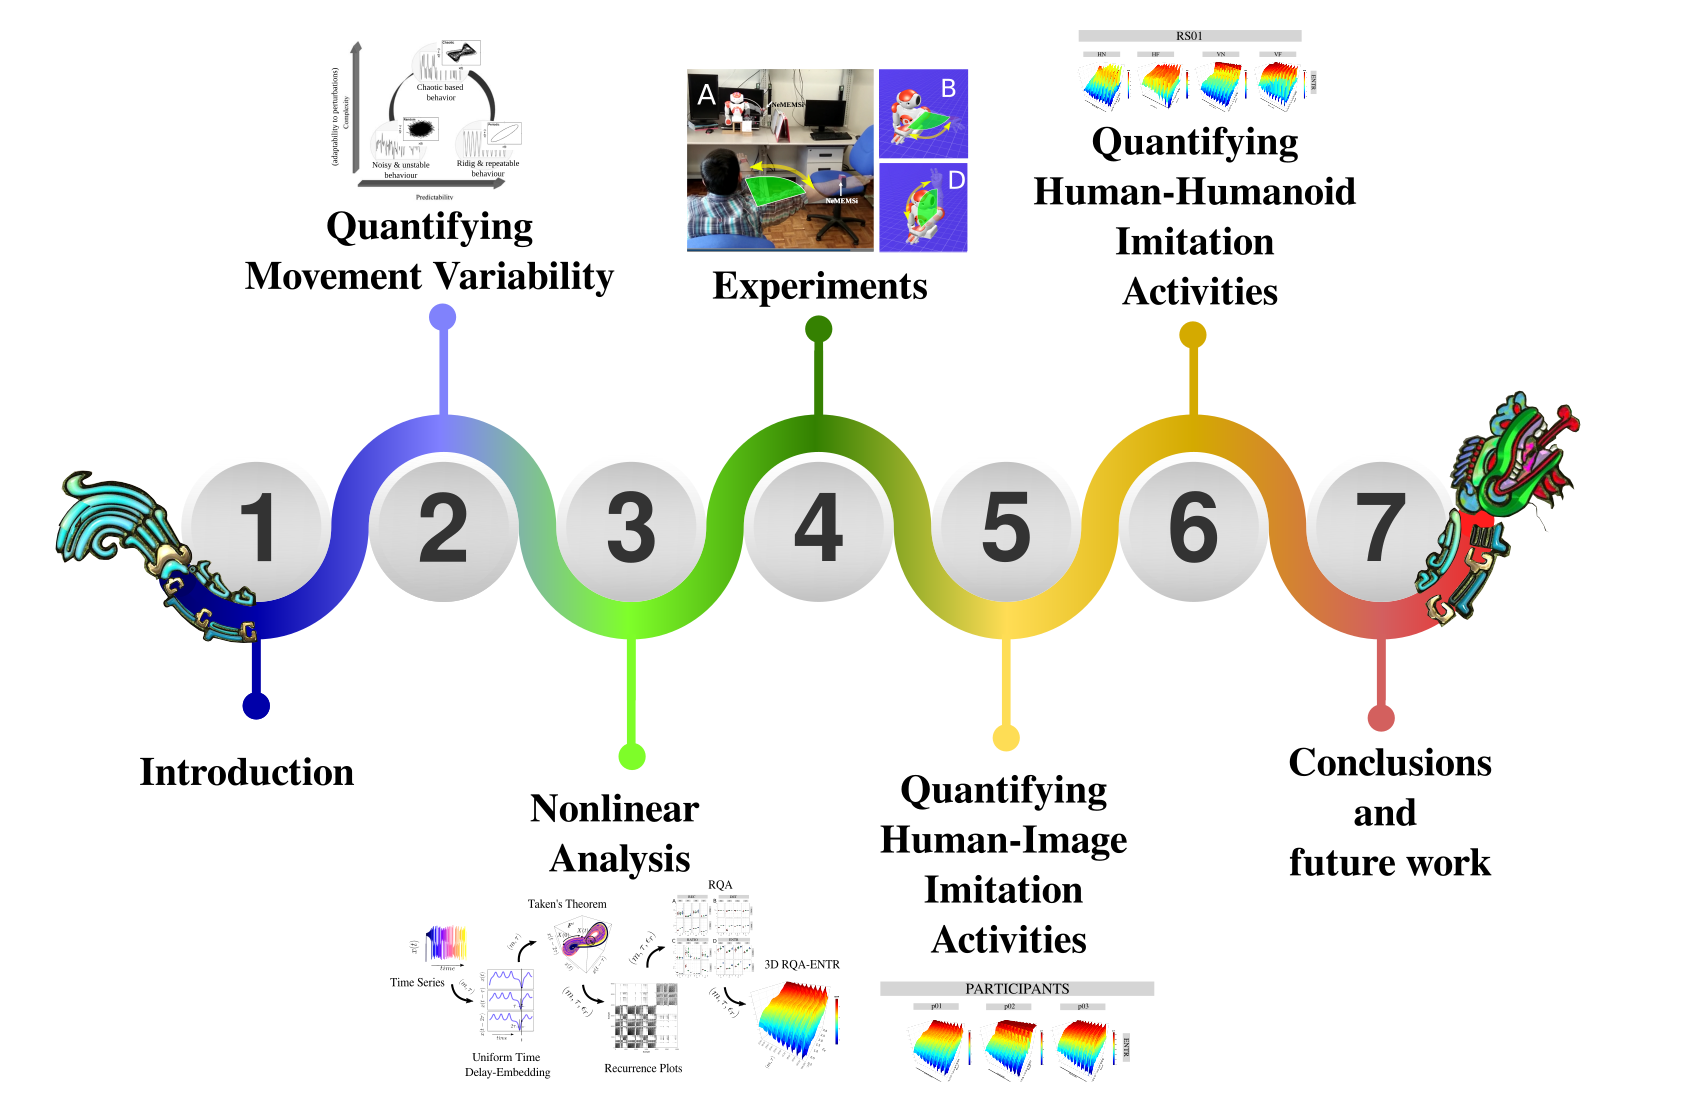
\includegraphics[width=0.8\linewidth]{./figs/oa-thesis/versions/drawing-v00.png}
        \caption{}
      \end{figure}
\end{frame}
}




{
\paper{\textbf{M. Xochicale 2019} GITHUB: https://github.com/air4children}
\begin{frame}{Artificial Intelligence and Robotics for Children}
    \vspace{-00mm}
      \begin{figure}
        \centering
        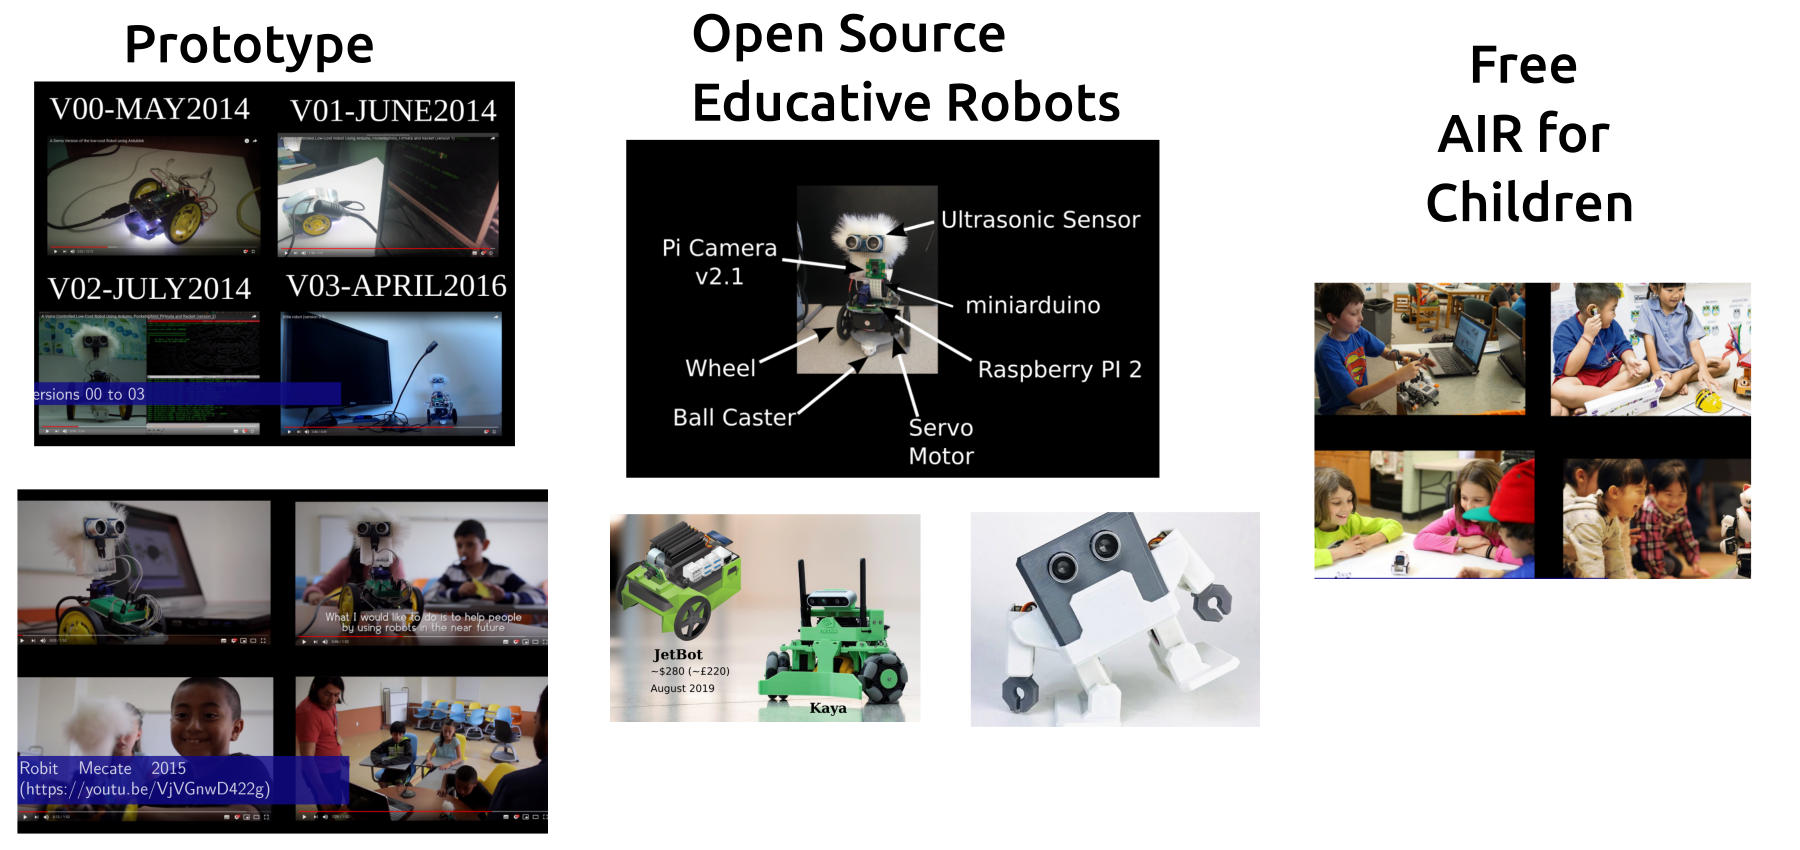
\includegraphics[width=0.99\linewidth]{./figs/air4children/versions/drawing-v00.png}
        \caption{}
      \end{figure}
\end{frame}
}


{
\paper{\textbf{Xochicale 2020} in Conf. of Reproducibility, Replicability and Trust in Science \faGithub github.com/mxochicale/rrts2020}
    \begin{frame}{Open-corTeX: ci framework for open scientific communication}

  \begin{columns}
    \begin{column}{.4\linewidth}
      \begin{itemize}
        \item Tools such as CI and containers can improve reproducibility
        \item The adoption of open-CorTeX might led to scientific outcomes 
	that are aligned to the principles of reproducibility, 
	inclusiviness, transparency, reusability and open accessibility.
      \end{itemize}
    \end{column}

  \begin{column}{.6\linewidth}
      \begin{figure}
        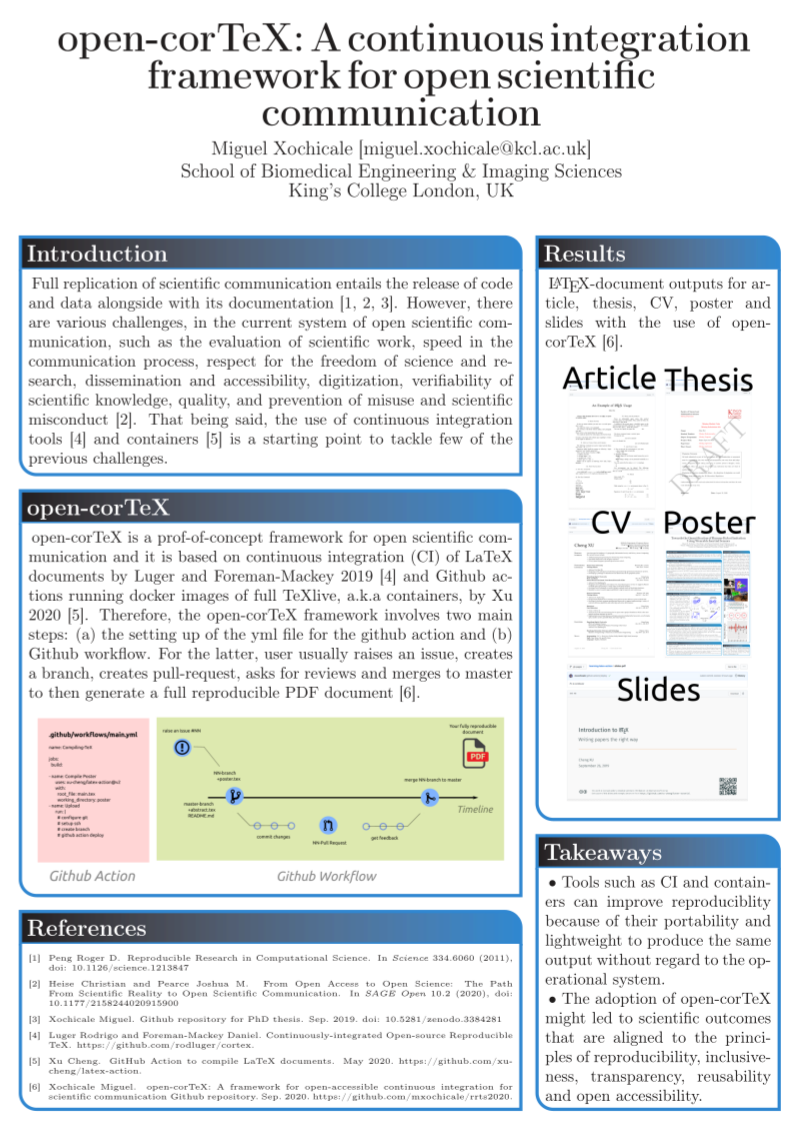
\includegraphics[scale=0.2]{./figs/open-cortex/versions/drawing-v00.png}
        \caption{}
      \end{figure}
    \end{column}
  \end{columns}
\end{frame}
}


